\documentclass[11pt,a4paper]{scrartcl}

\usepackage{fullpage}

%\usepackage[ngerman]{babel}
\usepackage[utf8]{inputenc}
\usepackage{graphicx}

\usepackage{amsmath}
\usepackage{amsthm}
\usepackage{mathtools}

\usepackage{listings}

%%%%% COMMANDS

\newcommand{\FT}{\mathcal{F}}
\newcommand{\T}{\mathrm{T}}
\newcommand{\IFT}{\mathcal{F}^{-1}}
\newcommand{\conv}{\ast}
\newcommand{\defined}{\coloneqq}

\newtheorem*{theorem}{Theorem}



\begin{document}

\title{Image Analysis Excercise Sheet 5}
\author{Markus Doering, 3153320}
\maketitle

\section{Background Subtraction in Video}
All python code for this excercise is found in file \verb$ia_05_01.py$ and in the appendix.
\stepcounter{subsection}
\subsection{Mean and Median Image}
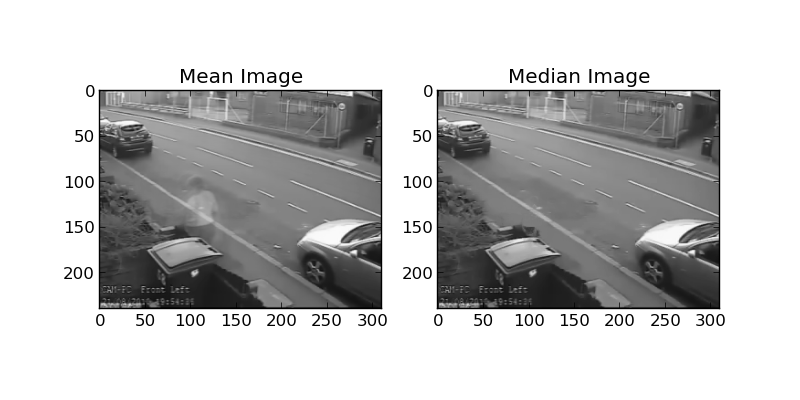
\includegraphics[width=.99\linewidth]{mean_and_median_image_cut.png}

\subsection{Subtracted Video}
The subtracted video can be found in the file \verb$left_is_mean_-_right_is_median.avi$.

\subsection{Median Subtraction}\label{median}
The Median Subtraction makes use of the underlying assumption that an object that is present in more than half of the analyzed frames is more likely to belong to the background rather than to the foreground. 
This can obviously lead to the wrong conclusions in border cases.

\subsection{Comparison of Mean and Median Subtraction}
The Mean Image averages each pixel over all frames, where in the Median Image each pixel is chosen from one particular fame. That makes the Mean Image more error prone in outlier situations, while 
it is more robust in very noisy videos. As seen in excercise \ref{median}, the Median Image labels all pixels as background that were left unchanged for at least half of the frames. There is no 
soft transition from foreground to background as in the Mean Image. 



\section{Cost Volume Filtering for Stereo}
All python code for this excercise is found in file \verb$ia_05_02.py$ and in the appendix. 

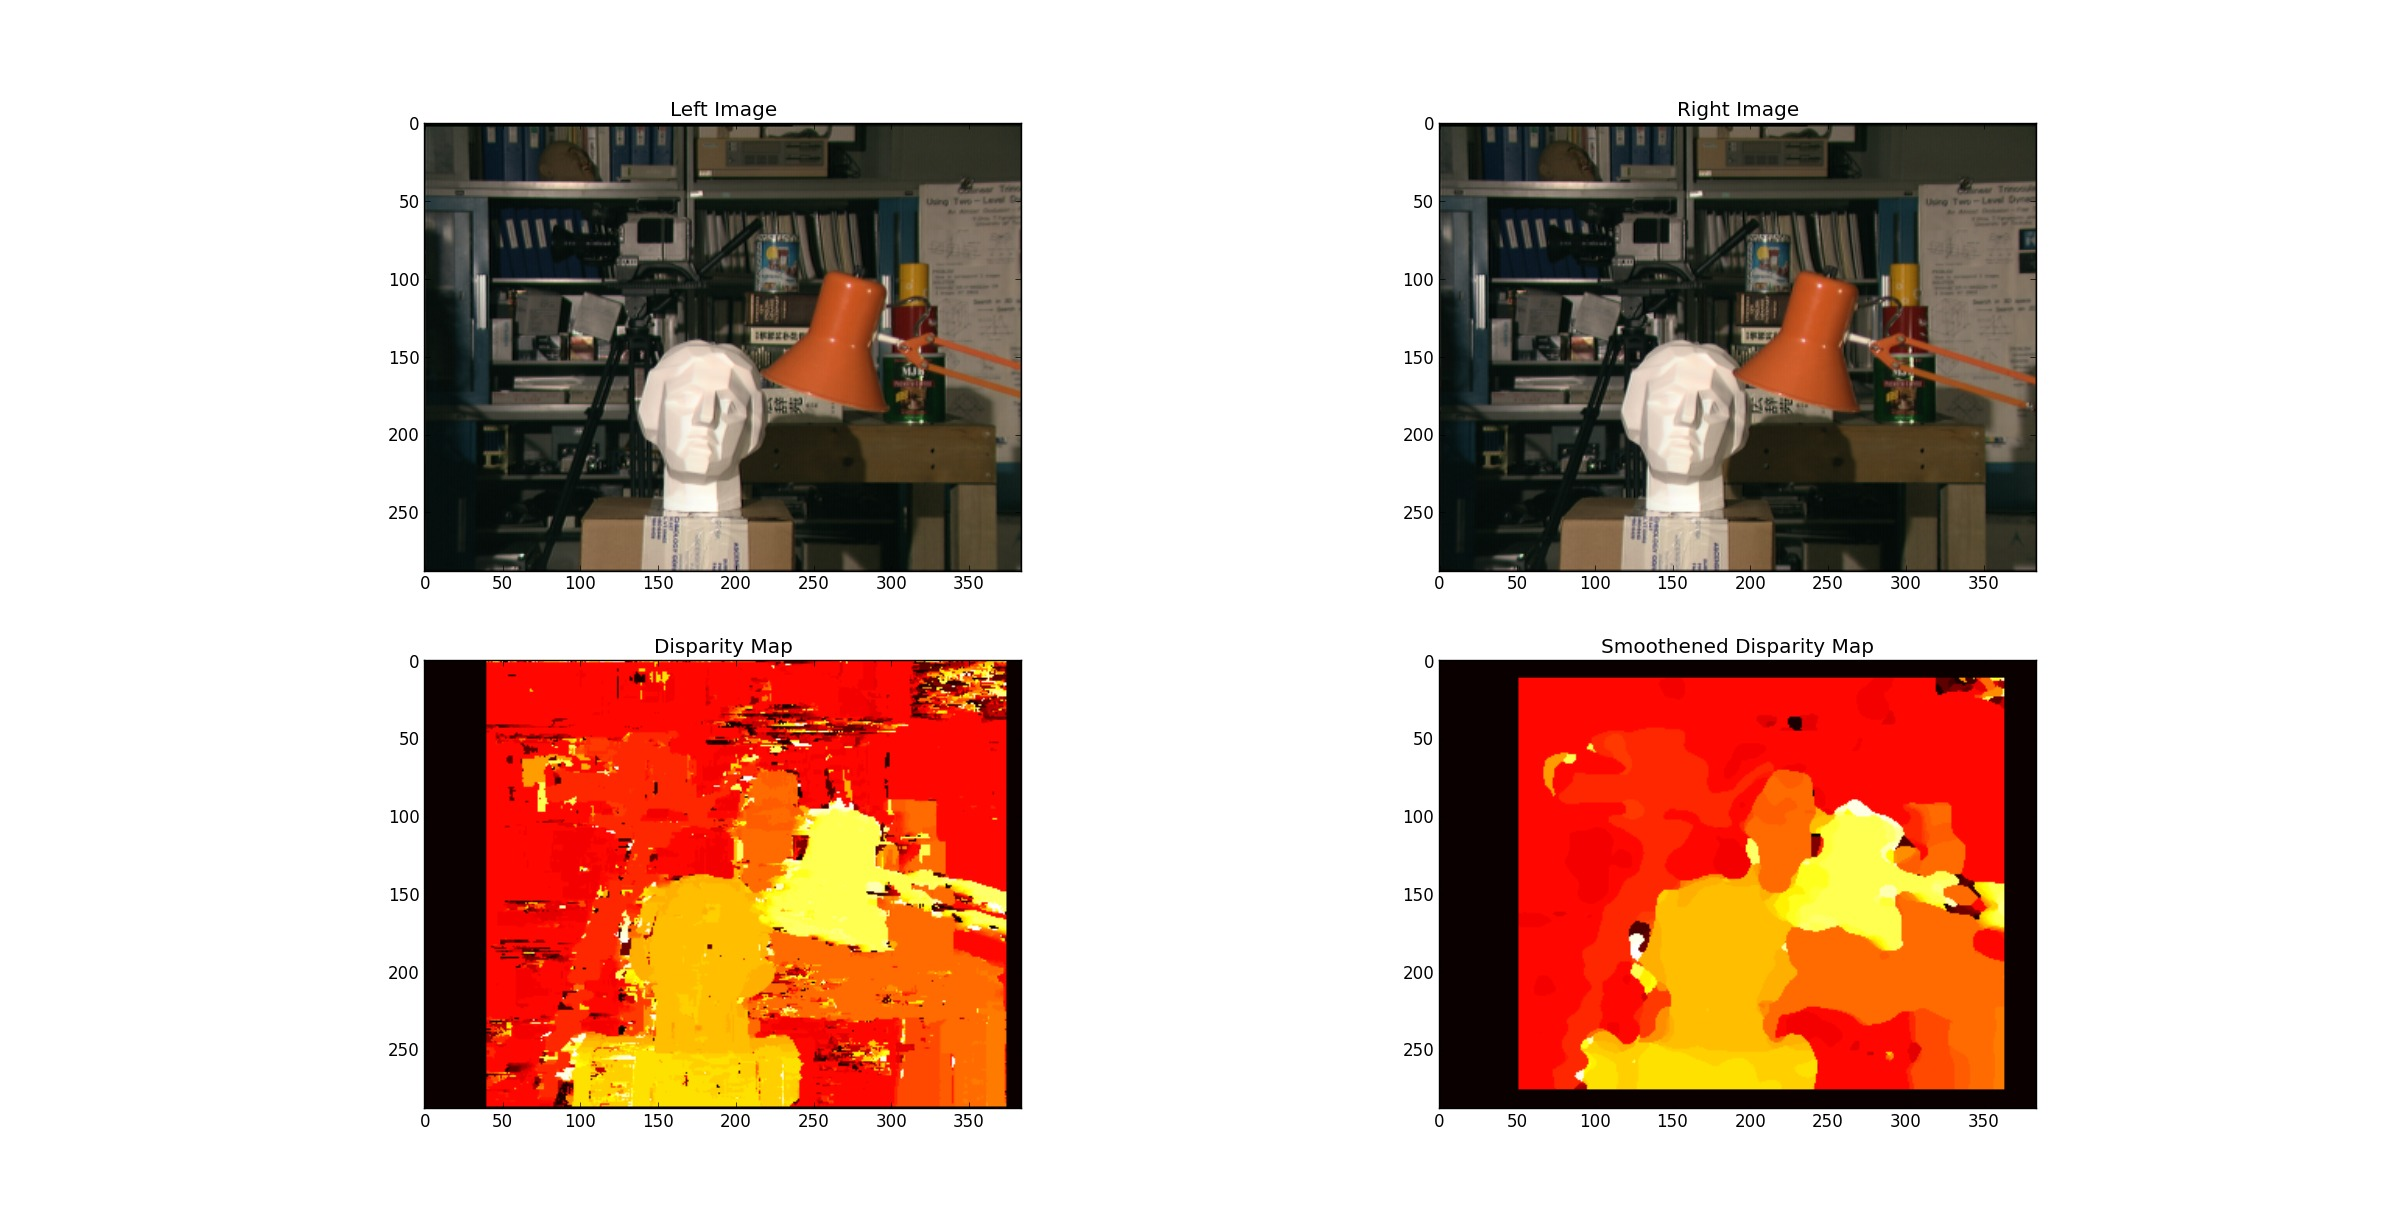
\includegraphics[width=.99\linewidth]{disparity_maps.jpg}

The original disparity map looks very rough and has many errors in areas of equal intensity, e.g. the upper right corner. The smoothened disparity map looks in fact smoother, but has also lost edge information. 
All in all the discovered disparity map gives an idea of the actual disparity, but is far from being perfect.

\newpage
\appendix
\lstinputlisting[language=python]{ia_05_01.py}
\newpage
\lstinputlisting[language=python]{ia_05_02.py}
\end{document}